\documentclass[../main.tex]{subfiles}

\begin{document}

\section{Elektrozwakke precisie testen}%
\label{sec:elektrozwakke_precisie_testen}

De eerste oplossing die aan bod is gekomen om de korte dracht van de zwakke wisselwerking te verklaren is de massa van het intermediaire boson.

\subsection{Zwakke uitwisselings deeltjes}%
\label{sub:zwakke_uitwisselings_deeltjes}

Zoals op het einde van vorig hoofdstuk is gezegd zijn de uitwisselings deeltjes van de zwakke interactie $W_1$, $W_2$ en $W_3$. De eerste 2 bosonen vormen samen de geladen zwakke stromen $W^\pm$. Hierbij was een voorspelling gedaan van de massa's van deze deeltjes enkele GeV te zijn. Wat is $W_3$ nu? Dit kan niet anders dan een neutraal deeltje zijn. Het eerste waar me dan aan denkt is het foton maar dit is niet mogelijk vanwege de koppeling met neutrinos. Er wordt gepostuleerd dat er ook een isospin singlet moet bestaan $B^0$ die ook neutraal is. Deze 2 kunnen opmengen tot $A^\mu$ en $Z^\mu$.
\begin{equation}
    \begin{aligned}
        \label{eq:zwakke_boson_opmenging}
        \begin{pmatrix}
            A^\mu\\
            Z^\mu
        \end{pmatrix}
        =
        \begin{pmatrix}
            \cos\theta_W & \sin\theta_W\\
            -\sin\theta_W & \cos\theta_W
        \end{pmatrix}
        \begin{pmatrix}
            B^0\\
            W^3
        \end{pmatrix}
    \end{aligned}
\end{equation}
$Z$ komt overeen met de zwakke wisselwerking en $A$ met de elektromagnetische. Wat een unificatie zal zijn tussen de zuivere zwakke bosonen en de elektrozwakke bosonen.

\subsection{Neutrale zwakke stroom}%
\label{sub:neutrale_zwakke_stroom}

De reden voor deze drang om een elektrozwakke unificatie te vinden stamt uit het vinden van de zuivere interactie stroom naast een axiale in de zwakke interactie experimenten (wat neerkomt op een zuivere vector stroom tussen specifieke chirale deeltjes). We hebben in deze 2 theorieën 2 uitwisselings deeltjes met gelijke kwantumgetallen die dan uiteraard zullen opmengen. De reden waarom de sterke wisselwerking niet bij wordt gehaald is omdat deze alleen met de quarks zal interageren en niet met de leptonen.\\
De elektrozwakke unificatie zegt ons dat er naast de geladen stromen ook een neutrale stroom zwakke stroom moet zijn  aan de hand van $Z^0$ uitwisseling. Het probleem is dat deze experimenteel nooit gezien worden. Deze zijn enkel zichtbaar als alle andere kanalen onderdrukt worden. Een mogelijke oplossing hiervoor is te werken met de neutrinos die alleen zwak kunnen interageren. In 1973 is in een bubbel experiment voor het eerst zo een neutrale stroom waargenomen en is dus aangetoond dat de neutrale stromen bestaan.

\subsection{Uitwisselings bosonen}%
\label{sub:uitwisselings_bosonen}

Nu we weten dat deze deeltjes bestaan willen we die natuurlijk ook effectief aanmaken. Om dit te doen hebben we ze in CERN de SPS-collider omgebouwd om $p\overline p$ verstrooiingen uit te voeren. De reden waarom we effectief $\overline p$ gebruiken is als we een antiquark uit $p$ moeten halen dat dit enkel een zeequark kan zijn en dus maar een kleine fractie van het proton zal hebben. Hierdoor is er niet genoeg energie om een $W$ boson aan te maken. Als je een $\overline p$ gebruikt zal het antiquark nu een veel grotere fractie van het proton hebben en we genoeg energie hebben om een $W$ boson aan te maken.
\begin{equation}
    \begin{aligned}
        \label{eq:w_productie}
        p + \overline p \rightarrow W + \text{rest} \rightarrow e\nu / \mu\nu + \text{rest}
    \end{aligned}
\end{equation}
Het maken van een anti protonenbundel is niet zo moeilijk. Schiet een protonenbundel op een target waar onderandere antiprotonen uit komen. Het probleem hierbij is dat deze alle richtingen uitgaan. Door een magneet in de buurt te zetten kan je deze colimeteren tot een bundel in een buis. Op dit moment divergeren de antiprotonen nog. Door deze af te koelen is het mogelijk om de antiprotonen allemaal in dezelfde richting te laten gaan. Door het heisenberg principe zal bij het samendrukken van de bundel in de ene richting deze in de andere richting uitzetten. De manier dat omzeilt kan worden is door causaliteit. Door he constant zijn van de lichtsnelheid is het mogelijk om in vogelvlucht informatie sneller aan de andere kant van de ring te krijgen en die informatie te gebruiken om de bundel bij te sturen.\\
Het probleem bij deze experimenten is dat de energie en momentum van de initiële quark en antiquark niet perfect geweten zijn. Het $W^+$ boson zal dus niet stil staan wat je niet kan meten. Wat we wel kunnen meten is de transversale impuls van het $W$ boson. Specifiek meten we $p_T(e)$ en omdat we met een hermetische detector werken is $p_T(\nu) = p_T(\text{missing}$. In de transversale richting is er geen boost en is $p_T$ dus Lorentz invariant. In het ruststelsel van $W$ is $|\vec{p}(e)|=-|\vec{p}(\nu)|$ en kunnen dus bepalen dat $p_T(e) = \frac{M_W}{2} \sin\theta^*$ met $\theta^*$ de de verval hoek in het ruststelsel.
\begin{equation}
    \begin{aligned}
        \label{eq:mom_dist}
        \frac{dn}{dp_T} &= \frac{dn}{d\theta^*} \frac{d\theta^*}{dp_T} \\
                        &= \frac{dn}{d\theta^*} \frac{1}{\sqrt{(M_W/2)^2-p^2}} 
    \end{aligned}
\end{equation}
Dit wil zeggen dat voor eender welke hoek afhankelijkheid er is in het aantal counts zullen we een piek waarnemen als $p_T=M_W/2$. Als we de transversale massa ($m_T=2p_T$) plotten in een histogram krijgen we dat de massa van het $W^+$ boson $M_W=80.0\pm 1.5$GeV is.

\begin{figure}[h]
    \centering
    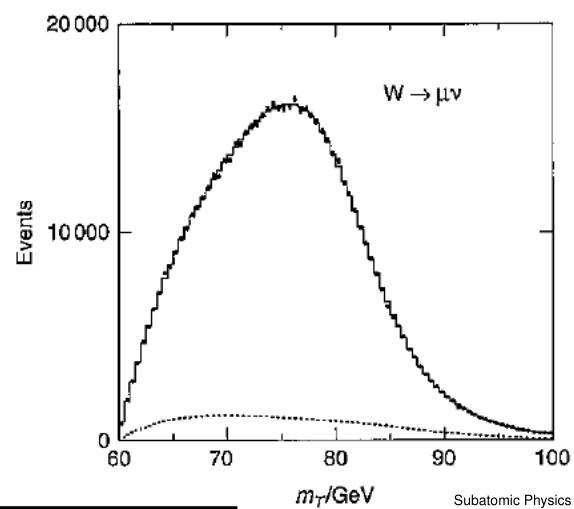
\includegraphics[width=0.3\linewidth]{elektroweak_precision_tests/w_boson_massa.png}
    \caption{Histogram van events in functie van de transversale massa}%
    \label{fig:elektroweak_precision_tests/w_boson_massa}
\end{figure}

Het meten van de massa van het $Z$ boson is een stuk makkelijker omdat we hier niet te maken hebben met een neutrino en de invariante massa rechtstreeks kunnen meten.
\begin{equation}
    \begin{aligned}
        \label{eq:z_productie}
        p + \overline p \rightarrow Z^0 + \text{rest} \rightarrow e^+/e^- (\mu^+/\mu^-) + \text{rest}
    \end{aligned}
\end{equation}
De massa van dit boson is $M_Z=91.5\pm 1.7$GeV.

\begin{figure}[h]
    \centering
    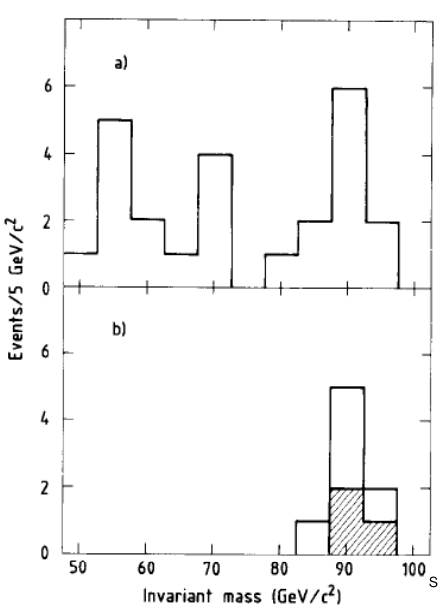
\includegraphics[width=0.3\linewidth]{elektroweak_precision_tests/z_boson_massa.png}
    \caption{Bepalen van de massa van het $Z$ boson}%
    \label{fig:elektroweak_precision_tests/z_boson_massa}
\end{figure}

\subsection{Spin van $W$}%
\label{sub:spin_van_w_}

\begin{figure}[h]
    \centering
    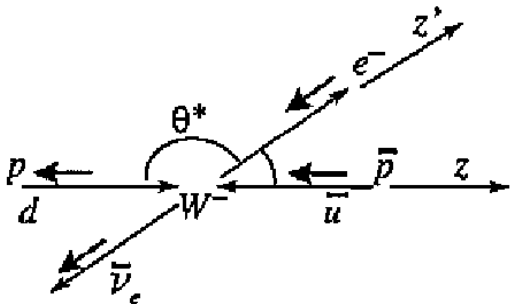
\includegraphics[width=0.4\linewidth]{elektroweak_precision_tests/spin_van_w.png}
    \caption{Schema van de kinematica van een verstrooiing om de spin van $W$ te bepalen}%
    \label{fig:elektroweak_precision_tests/spin_van_w}
\end{figure}

Nemen we aan de V-A theorie correct is en we laten een anti-up in in een down quark annihileren tot een $W^-$ boson. V-A zegt dat $d$ een linkshandig deeltje moet zijn en zijn spin is dus antiparallel aan de bewegingsrichting. Voor $\overline u$ zegt V-A dat dit een rechtshandig deeltje is en ligt zijn spin parallel aan zijn bewegingsrichting. De spin van $W^-$ is de combinatie van de 2 spins, $J=1$ en $J_z=-1$. De $-1$ projectie op de de z-richting is door conventie dat de z-richting gelijk wordt gesteld aan de proton richting. Vervolgens laten we $W^-$ vervallen naar de een $e^-$ en $\overline \nu$. Omdat we met een elektron te maken hebben weten we dat het intermediaire boson een $W^-$ boson zal zijn. Voor de uitgaande deeltjes kunnen we nu ook als een kwantisatieas zien met $e^-$ linkshandig en $\overline \nu$ rechtshandig. Dit geeft ons terug een projectie van de spin op deze as $J_{z'}=-1$. We moeten dus de waarschijnlijkheid bepalen waarbij $J_z=-1$ wordt omgezet in $J_{z'}=-1$. Dit gebeurt aan de hand van de rotatie matrices.
\begin{equation}
    \begin{aligned}
        \label{eq:kans_proj_omz}
        \frac{d\sigma}{d\Omega} &\propto (d_{-1,-1}^1)^2\\
                                &\propto \left[ \frac{1}{2} (1+\cos\theta^*)\right]^2
    \end{aligned}
\end{equation}
Kijken we nu experimenteel naar de hoekdistributie zien we duidelijk dat het $W^-$ een spin van 1 moet hebben.

\begin{figure}[h]
    \centering
    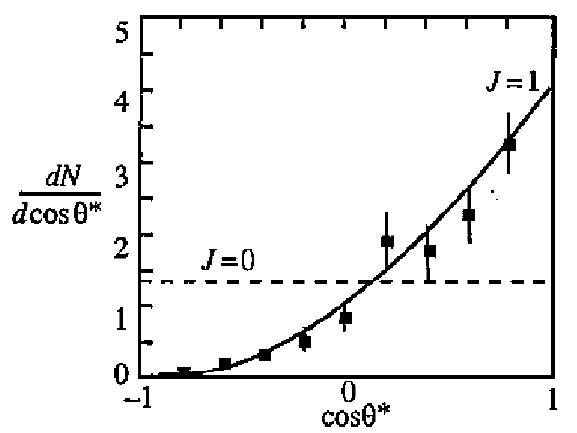
\includegraphics[width=0.4\linewidth]{elektroweak_precision_tests/spin_van_w_resultaten.png}
    \caption{Experimentele resultaten van de spin van $W$}%
    \label{fig:elektroweak_precision_tests/spin_van_w_resultaten}
\end{figure}

\subsection{Elektrozwakke unificatie}%
\label{sub:elektrozwakke_unificatie}

Kijken we nu terug naar de stromen van de geladen zwakke interactie.
\begin{equation}
    \begin{aligned}
        \label{eq:stroom_geladen_zwakke_int}
        \begin{matrix}
            W^\pm = \frac{1}{\sqrt{2}} (W^1\pm iW^2) & j^\pm = \frac{1}{\sqrt{2}} (j_1\pm ij_2) \\
            j_\mu^- = \overline\nu_{eL}\gamma_\mu e_L^- & j_\mu^+ = \overline e_L^-\gamma_\mu\nu_{eL}
        \end{matrix}
    \end{aligned}
\end{equation}
De zwakke interactie heeft 3 intermediaire bosonen, het 3de boson is een isocalaire interactie $B$. De $SU(2)$ groep kunnen we unificeren tot $SU(2)\otimes U(1)$. $U(1)$ is hier niet de elektromagnetische groep omdat $B$ niet exact het foton kan zijn. Voor die wisselwerking is de zwakke hyperlading toegevoegd $Y_W = 2(Q-I_z)$. Een aantal voorbeelden van de zwakke hyperlading zijn gegeven in tabel \ref{tab:zwakke_hyperlading}.

\begin{table}[h]
    \centering
    \caption{Voorbeelden van de hyperlading}
    \label{tab:zwakke_hyperlading}
    \begin{tabular}{cccc}
                & $Y_W$ &       & $Y_W$ \\
        \hline
        $\nu_L$ & -1    & $u_L$ & $\frac{1}{3}$\\
        $l_L^-$ & -1    & $d_L$ & $\frac{1}{3}$\\
                &       & $u_R$ & $\frac{4}{3}$\\
        $l_R^-$ & -2    & $d_R$ & $-\frac{2}{3}$\\

    \end{tabular}
\end{table}

Mengen we nu $W_3$ en $B$ op dan krijgen we 
\begin{equation}
    \begin{aligned}
        \label{eq:w_b_mixing}
        \begin{pmatrix}
            Z^0\\
            A
        \end{pmatrix}
        &= \frac{1}{\sqrt{g^2+g'^2}} 
        \begin{pmatrix}
            g & -g'\\
            g' & g
        \end{pmatrix}
        \begin{pmatrix}
            W_3\\
            B
        \end{pmatrix}\\
        &=
        \begin{pmatrix}
            \cos\theta_W & -\sin\theta_W\\
            \sin\theta_W & \cos\theta_W
        \end{pmatrix}
        \begin{pmatrix}
            W_3\\
            B
        \end{pmatrix}
    \end{aligned}
\end{equation}
met $g$ de zwakke koppelingsconstante en $g'$ de koppelingsconstante die we niet kennen waarmee $B$ aan de zwakke hyperlading koppelt. De weinberg hoek kan geschreven worden als: $\theta_W\equiv \tan^{-1} \frac{g'}{g}$. Nu wordt de Lagrangiaan gegeven door:
\begin{equation}
    \begin{aligned}
        \label{eq:elektozwakke_lagrangiaan}
        \mathcal{L} &= g(j_\mu^1W_1^\mu+j_\mu^2W_2^\mu+j_\mu^3W_3^\mu)+ \frac{g'}{2} j_\mu^YB^\mu\\
                    &= \frac{g}{\sqrt{2}} (j_\mu^-W_+^\mu+j_\mu^+W_-^\mu) + j_\mu^3(gW_3^\mu-g'B^\mu) 6 g'j_\mu^{EM}B^\mu\\
                    &= \frac{g}{\sqrt{2}} (j_\mu^-W_+^\mu+j_\mu^+W_-^\mu) + \frac{g}{\cos\theta_W} (j_\mu^3 - \sin^2\theta_Wj_\mu^{EM})Z^\mu + g\sin\theta_Wj_\mu^{EM}A^\mu
    \end{aligned}
\end{equation}
Hierbij kunnen we mooi zien in de eerste lijn dat de $W$'s interageren met een strekte $g$ en $B$ met een sterkte $g'$. Als we ervan uit gaan dat $A$ een foton beschrijft moet $g\sin\theta_W \propto e$ zijn of exact $g\sin\theta_W = \sqrt{4\pi\alpha}$. We zien dus eigenlijk dat g zo  goed als gelijk is aan de elektromagnetische koppeling. Uit de 2de term krijgen we de koppelingsterkte van het $Z$ boson.
\begin{equation}
    \begin{aligned}
        \label{eq:koppeling_z}
        g_Z &= \frac{g}{\cos\theta_W} (I_z - Q\sin^2\theta_W)\\
            &= \frac{g}{\cos\theta_W} c_Z\\
            c_Z = I_z - Q\sin^2\theta_W
    \end{aligned}
\end{equation}
Hier is $c_Z$ equivalent met de kleurfactoren van QCD. Ten laatste voor de $W$ koppeling moet deze $g$ overeen komen met de propagator term uit de klassieke theorie
\begin{equation}
    \begin{aligned}
        \label{eq:koppeling_w}
        G_F = \frac{\sqrt{2}g^2}{8M_W^2} 
    \end{aligned}
\end{equation}
In de propagator term komt de massa van het $W$ boson voor:
\begin{equation}
    \begin{aligned}
        \label{eq:massa_w}
        M_W &= \frac{g^2\sqrt{2}}{8G_F} \\
            &= \sqrt{ \frac{\pi\alpha}{\sqrt{2}G_F}} \frac{1}{\sin\theta_W} = \frac{37.3}{\sin\theta_W} \text{GeV}
    \end{aligned}
\end{equation}
Zo is het mogelijk om de elektromagnetische en zwakke wisselwerking op te schrijven in 2 constantes: $\alpha$ en $\theta_W$.

\end{document}
